\documentclass{standalone}


\usepackage{pgfplots, tikz}
\usetikzlibrary{calc,fadings,decorations.pathreplacing}
\usetikzlibrary{fit, arrows, shapes, shapes.geometric, fadings, shapes.arrows, shadows}
\usepackage{relsize}

\begin{document}


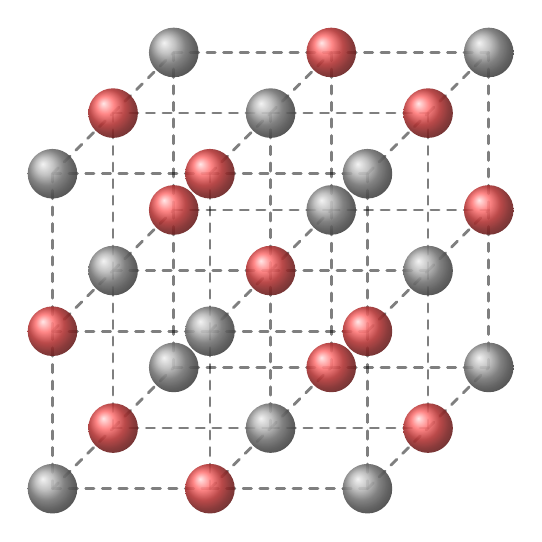
\begin{tikzpicture}[line cap=round,line join=round,>=triangle 45,x=1.0cm,y=1.0cm,scale=1]
\tikzset{>=latex}
\def\ballradius{0.45}
\def \dx{2};
\def \dy{2};
\def \dz{2};
\def \nbx{3};
\def \nby{3};
\def \nbz{3};

% z lines
\foreach \x in {1,...,\nbx} {
    \foreach \z in {1,...,\nbz}{
        \foreach \y in {2,...,\nby}{
            \draw [-, dashed, line width = 1pt, opacity=0.5]( \x*\dx , \y*\dy, \z*\dz) -- (\x*\dx,\y*\dy - \dy,\z*\dz);
        }
    }
}

% x lines
\foreach \y in {1,...,\nbx} {
    \foreach \z in {1,...,\nbz}{
        \foreach \x in {2,...,\nbx}{
            \draw [-, dashed, line width = 1pt, opacity=0.5](\x * \dx - \dx,\y*\dy,\z*\dz) -- ( \x * \dx,\y*\dy,\z*\dz);
        }
    }
}

% y lines
\foreach \x in {1,...,\nbx} {
    \foreach \y in {1,...,\nbz}{
        \foreach \z in {2,...,\nby}{
            \draw [-, dashed, line width = 1pt, opacity=0.5] ( \x*\dx,\y*\dy,\z*\dz) -- (\x*\dx,\y*\dy,\z*\dz - \dz);
        }
    }
}



\foreach \x in {1,...,\nbx} {
    \foreach \y in {1,...,\nby} {
        \foreach \z in {1,...,\nbz} {
			     
			
			\ifodd\numexpr\x+\y+\z\relax
			\def\Color{gray!70}
			\else
			\def\Color{red!70}
			\fi
			\shade[ball color=\Color, opacity=0.9] (\x*\dx,\y*\dy,\z*\dz) circle(0.7*\ballradius);

        }
    }
}

			

\end{tikzpicture}

\end{document}
